
\documentclass[12pt]{article}
\usepackage[utf8]{inputenc}
\usepackage{float}
\usepackage{amsmath}


\usepackage[hmargin=3cm,vmargin=6.0cm]{geometry}
%\topmargin=0cm
\topmargin=-2cm
\addtolength{\textheight}{6.5cm}
\addtolength{\textwidth}{2.0cm}
%\setlength{\leftmargin}{-5cm}
\setlength{\oddsidemargin}{0.0cm}
\setlength{\evensidemargin}{0.0cm}

%misc libraries goes here
\usepackage{bytefield}
\usepackage{tikz}

\begin{document}

\section*{Student Information }
%Write your full name and id number between the colon and newline
%Put one empty space character after colon and before newline
Full Name : Hakan Bostan \\
Id Number : 2098812


% Write your answers below the section tags
\section*{Package Definition}

Before writing our codes we discussed what kind of packet structure to use. We decided on a packet with 10 bytes header and a 256 byte (at most) data section.\\
\begin{center}
\begin{bytefield}[bitwidth=1.1em]{32}
\bitbox{6}{from/to/ack} & \bitbox{9}{timestamp} & \bitbox{5}{datalength} & \bitbox{12}{data}\\
\bitbox[t]{8}{$\underbrace{\hspace{22em}}_{\text{\normalsize Header}}$}
\end{bytefield}
\end{center}

\textbf{from/to/ack: } 1 byte, this field holds the source, destination and acknowledgement flag. Acknowledgement flag is used to determine whether a packet is a data packer or an acknowledgement packet. We have 5 nodes, A,B,C,D,E, and we mapped them to 0,1,2,3,4. 'from' and 'to' is a number in [0,4] range. Also acknowledgement flag is 0 or 1. We calculated a number with (source)+(destination)*5+(ack)*25 formula (i.e. in radix 5 representation). This number is guaranteed to be smaller than 256 so we can store it in a byte safely.\\

\textbf{timestamp: } 8 bytes, this field holds the time at the moment that the packet is created. This field is then later used to calculate end to end delay at destination.\\

\textbf{datalength: } 1 byte, this field holds the size of the following data part in bytes.\\

\textbf{data: } 256 bytes max., this field holds the data to be sent to the destination. Since we used only one byte in header to represent the size of data, data's size cannot be greater than 256 bytes.

\section*{Routing Tables}
\begin{center}
\begin{tabular}{|cc|}
\hline
\multicolumn{2}{|c|}{\textbf{0 (A)}}\\
\hline
\textbf{Destination} & \textbf{Send To}\\
0 & - \\
1 & 1 \\
2 & 1 \\
3 & 1 \\
4 & 1 \\
\hline
\end{tabular}
\bigskip
\begin{tabular}{|cc|}
\hline
\multicolumn{2}{|c|}{\textbf{1 (B)}}\\
\hline
\textbf{Destination} & \textbf{Send To}\\
0 & 0 \\
1 & - \\
2 & 2 \\
3 & 2 \\
4 & 2 \\
\hline
\end{tabular}
\bigskip
\begin{tabular}{|cc|}
\hline
\multicolumn{2}{|c|}{\textbf{2 (C)}}\\
\hline
\textbf{Destination} & \textbf{Send To}\\
0 & 1 \\
1 & 1 \\
2 & - \\
3 & 3 \\
4 & 3 \\
\hline
\end{tabular}

\begin{tabular}{|cc|}
\hline
\multicolumn{2}{|c|}{\textbf{3 (C)}}\\
\hline
\textbf{Destination} & \textbf{Send To}\\
0 & 2 \\
1 & 2 \\
2 & 2 \\
3 & - \\
4 & 4 \\
\hline
\end{tabular}
\bigskip
\begin{tabular}{|cc|}
\hline
\multicolumn{2}{|c|}{\textbf{4 (D)}}\\
\hline
\textbf{Destination} & \textbf{Send To}\\
0 & 3 \\
1 & 3 \\
2 & 3 \\
3 & 3 \\
4 & - \\
\hline
\end{tabular}\\
\end{center}

Since we used 0,1,2,3,4 to represent the machines, we also needed a way to get the IPs of the machines. Machines have to interfaces but they can only see eachother over only one of them, so we just needed to store only one of the two IPs each machine has. We stored these IPs as (target,this,ip) tuple. This tuple roughly translates to 'ip' of 'target' which is reachable from 'this' machine is this.\\

For routing, we used a similar notation, (Destination,Source,SendTo). We can reach the Destionation from Source by first going to SendTo. Also IP of SendTo can be found from IP table.

\section*{Measurements}
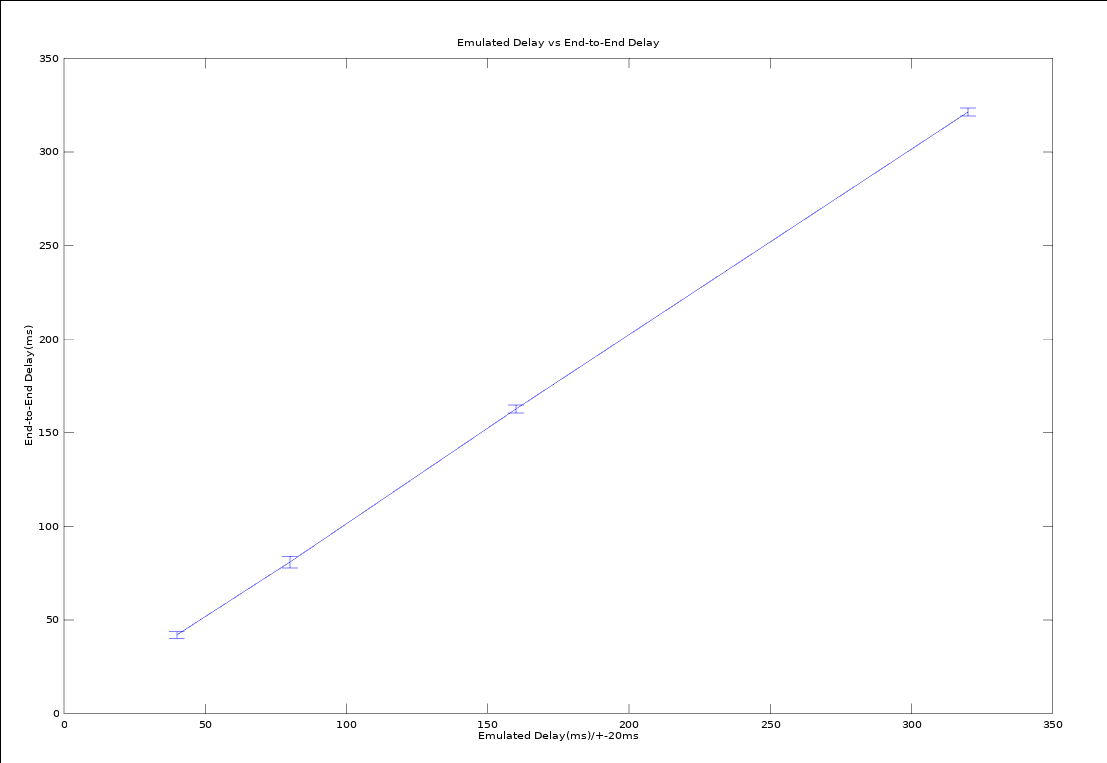
\includegraphics[height=360pt]{image.png} \\

There is a linear relation between emulated delay and end-to-end delay. But since the emulated delay doesn't include quing delay, propagation delay, transmission delay and routing delay. This leads to slope of the line being greater than one. Moreover, delays we introduced with 'tc' command dominate these mentioned delays, therefore the graph is still linear.\\

To measure the end to end delay we put a timestamp to the packet to be sent while we create it, and when the destiantion receives the package it extracts this timestamp and measures the time passed, giving us the end-to-end delay. For this method to work, we first needed to synchronize the clocks of the hosts. In order to do this we setup a NTP(Network Time Protocol) server on E and added A as peer. After syncing clocks of A and E we used the diffclock tool to check if something is wrong and we got 0/0ms difference. We are now confident that our method works as intended.\\

To calculate the end-to-end delay values we sent 100 packets from A to E and get the average of those times. Averages for 10ms, 20ms, 40ms, 80ms network delays are, 42.0280623436ms, 80.9206318855ms, 162.675359249ms, 321.32212162ms respectively. After getting the averages we calculated the \%95 confidence interval by multiplying the standard deviation by 1.96 and dividing it by 10. Our confidence intervals are 42.0280623436$\pm$ 1.84840390578ms, 80.9206318855$\pm$3.1282490074ms, 162.675359249$\pm$2.11410422494ms, 321.32212162$\pm$2.07671289966ms respectively. We then used octave to plot the grap.\\

During homework, we designed and implemented all the parts together.


\end{document}